\section{Uniform Scalar Quantizer}
In this part we implement the most basic quantizer. The USQ is entirely defined with three parameters:\begin{itemize}
\item $n_{bits}$, the number of bits used to code one sample. $2^{n_{bits}}$ is the number of output value;
\item m, the mean of the output values;
\item xmax the maximum of the output values;
\end{itemize}

In this part we tried m=0 and m=1.5. The result that we got plotting the input sigal versus the input signal is presented on figure \ref{USQ_INOUT}.

\begin{figure}[!h]
  \centering
\subfloat[m = 0]{  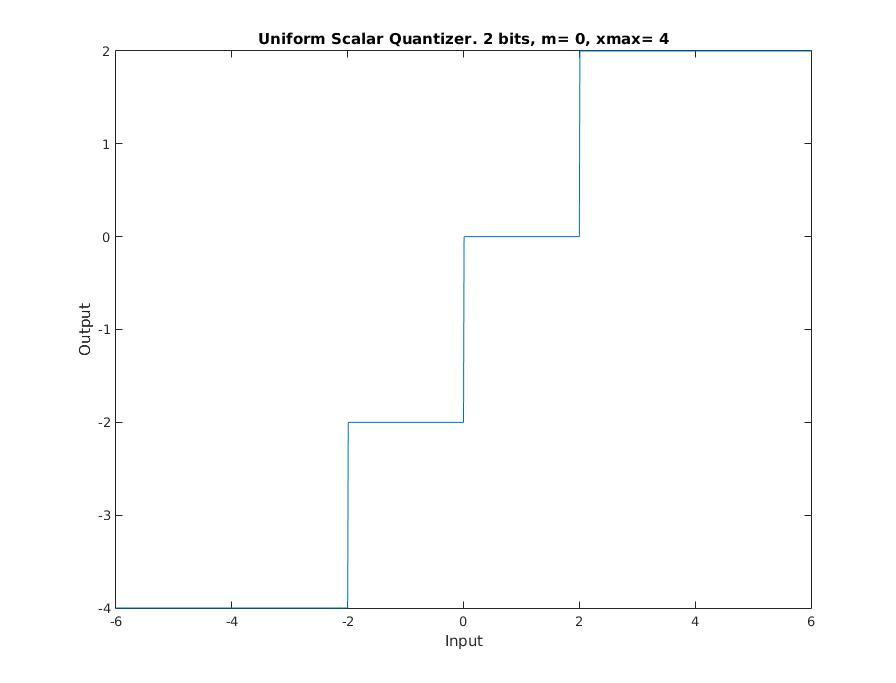
\includegraphics[scale=.3]{USQ_INOUT_m0} }
\subfloat[m = 1.5]{  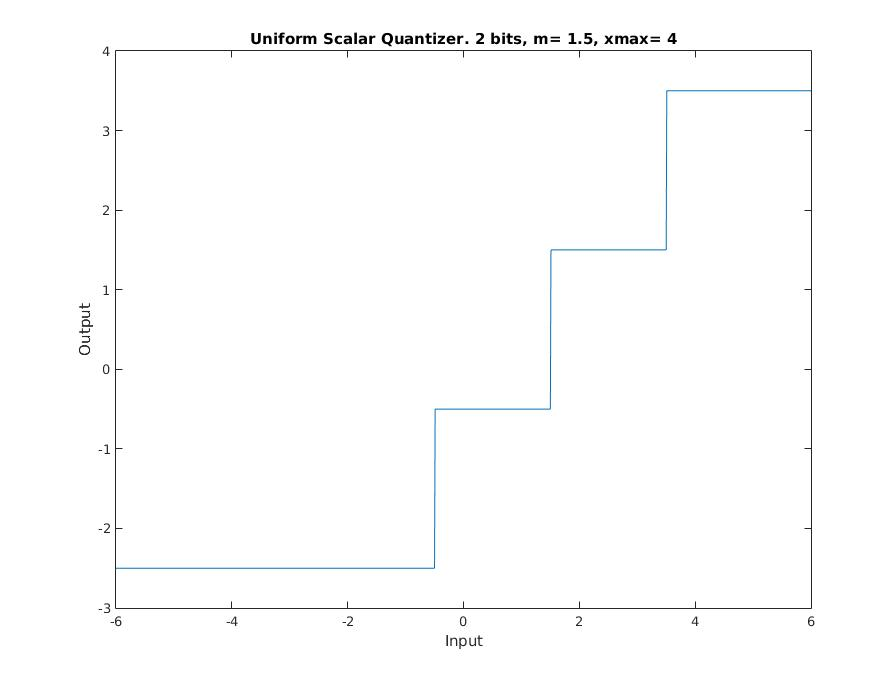
\includegraphics[scale=.3]{USQ_INOUT_m15} }

  \caption{Input vs Output}
  \label{USQ_INOUT}
\end{figure}
To compare the two settings, we need to plot the distorsion-rate curve and compare the performance. This is presented on figure \ref{USQ_RateDistCurve}.

\begin{figure}[!h]
  \centering
  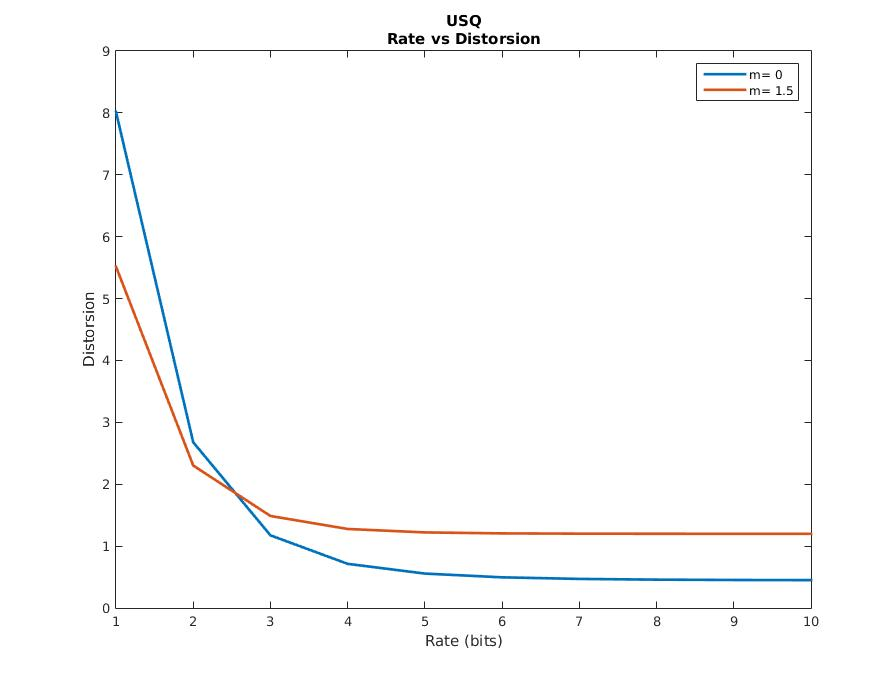
\includegraphics[scale=.35]{USQ_RateDistCurve}
  \caption{Rate-Distorsion curve for two values of m.}
  \label{USQ_RateDistCurve}
\end{figure}

%%% Local Variables:
%%% TeX-master: "master"
%%% End: